\documentclass[16pt]{beamer}

\usepackage[utf8]{inputenc}
\usepackage{hyperref}
\usepackage{times}
\usepackage{graphicx}
\usepackage[english]{babel}
%\usepackage[onehalfspacing]{setspace}
\usepackage{amsmath}
\setbeamertemplate{section in toc}[sections numbered]
\setbeamertemplate{subsection in toc}[subsections numbered]
\usepackage{bm}


%Information to be included in the title page:
\title{Diffusion Quantum Monte Carlo With Gaussian Trial Wave Functions}
\subtitle{Calculating Anharmonic Zero Point Energies}
\author{Simon Neidhart}
\institute{Department of Physics, University of Basel}
\date{\today}


\begin{document}
\frame{\titlepage}

\begin{frame}
\frametitle{Table of Contents}
\tableofcontents
\end{frame}

\section{Introduction}
\begin{frame}
\frametitle{Introduction}
\begin{itemize}
\item Diffusion quantum Monte Carlo (DQMC) solves the Schrödinger equation and gives the quantum-mechanical ground state energy to calculate the zero point energy (ZPE).
\item We use Gaussian guiding wave function to improve the convergence.
\item DFTB+ is used for calculation the energy.
\item The goal is to improve the harmonic approximation for the ZPE
\end{itemize}
\end{frame}

\section{The DQMC Algorithm}
\begin{frame}
\frametitle{The Unguided DQMC Algorithm}
\begin{itemize}
\item The stationary solution of the diffusion equation satisfies the Schrödinger equation and has the propagator $G(\bm{x},\bm{y};\Delta \tau) = \frac{1}{\sqrt{2 \pi \Delta \tau}} e^{-(\bm{x}-\bm{y})^2/(2\Delta \tau)} e^{-\Delta \tau (V(\bm{y}) - E_T)}$.
\item We simulate a ensemble of walkers to reach this stationary solution and the Schrödinger equation is solved.
\item The propagator consists of a diffusion term $\frac{1}{\sqrt{2 \pi \Delta \tau}} e^{-(\bm{x}-\bm{y})^2/(2\Delta \tau)}$ and a branching term $e^{-\Delta \tau (V(\bm{y}) - E_T)}$.
\item The diffusion term is simulated by randomly displacing the walker from its previous position according to a Gaussian distribution.
\item The branching term updates the weight of a walkers according to which the walker survives, reproduces or dies.
\item The trial energy $E_T$ is then adjusted to keep the population of walkers stable.
\item With time, the trial energy $E_T$ converges to the solution of the Schrödinger equation.
\end{itemize}
\end{frame}

\section{The Guiding Wave Function}
\begin{frame}
\frametitle{The Guiding Wave Function}
\begin{itemize}
\item We use the harmonic approximation of the potential energy surface with the Hessian matrix.
\item Gaussian guiding wave functions $\psi_T(x) = \mathcal{N} e^{-x^2/(2 \sigma^2)}$ along are placed the normal modes.
\item The width of the Gaussian is given by $\sigma^2 = \frac{1}{\omega m}$, where $\omega^2$ is the corresponding eigenvalue of the Hessian matrix.
\item This extends the algorithm with a drift velocity $\bm{v}(\bm{x}) = \nabla_{\bm{x}} \psi_T(\bm{x})$ which is added to the pure diffusion and a kinetic energy term in the local energy $E_L(\bm{x}) = (H\psi_T(\bm{x}))/\psi_T(\bm{x})$ which replaces the potential energy in the branching step.
\item With Gaussian trial wave functions, we can calculate the drift velocity and the local energy analytically.

\end{itemize} 

\end{frame}

\begin{frame}
\frametitle{The Guiding Wave Function}
\begin{center}
\scalebox{0.35}{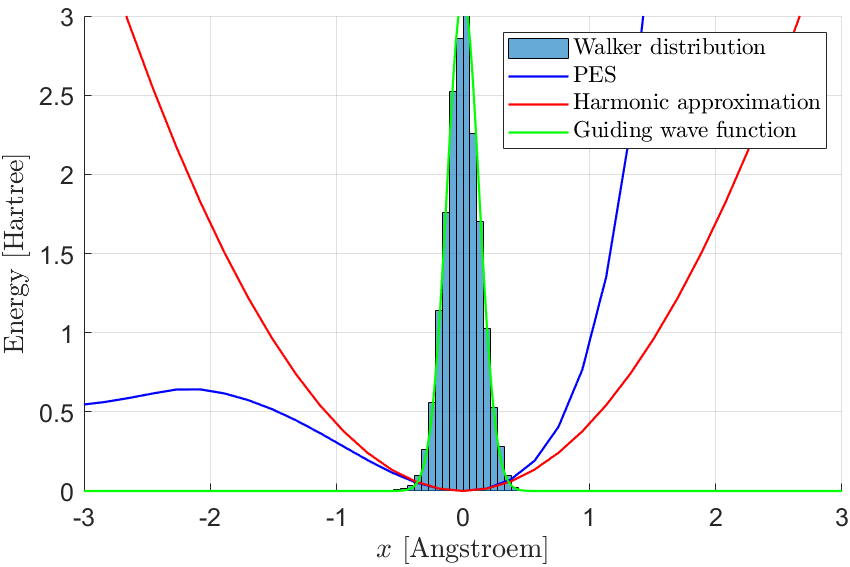
\includegraphics{walkers2.png}}\\
Fig. 1. Typical dimension in the coordinate system of the normal modes.
\end{center}

\end{frame}

\section{Input and Output}
\begin{frame}
\frametitle{Input and Output}
Input:\\
\begin{itemize}
\item Equilibrium geometry of the atoms (must not be perfect as geometry will be optimized by DFTB+ in the beginning)
\item Masses of the atoms
\end{itemize}
Output:
\begin{itemize}
\item Zero point energy
\item The walker distribution give a sample of the nucleonic wave function
\end{itemize}
\end{frame}

\section{Results}

\subsection{$C_2 H_6$}
\begin{frame}
\frametitle{Results}
\framesubtitle{$C_2 H_6$ (first test case)}
\begin{center}
\scalebox{0.40}{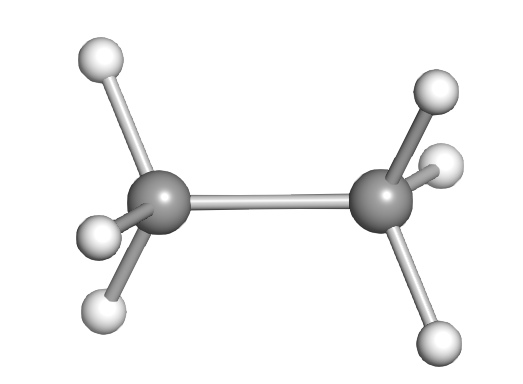
\includegraphics{p1.png}}\\
Fig. 2. Input structure of Ethane
\end{center}
First test case to develop the algorithm and check the result with a literature value.
\end{frame}

\begin{frame}
\frametitle{Results}
\framesubtitle{$C_2 H_6$}
10 simulations with 1000 walkers for 10000 time steps
\begin{center}
\scalebox{0.2}{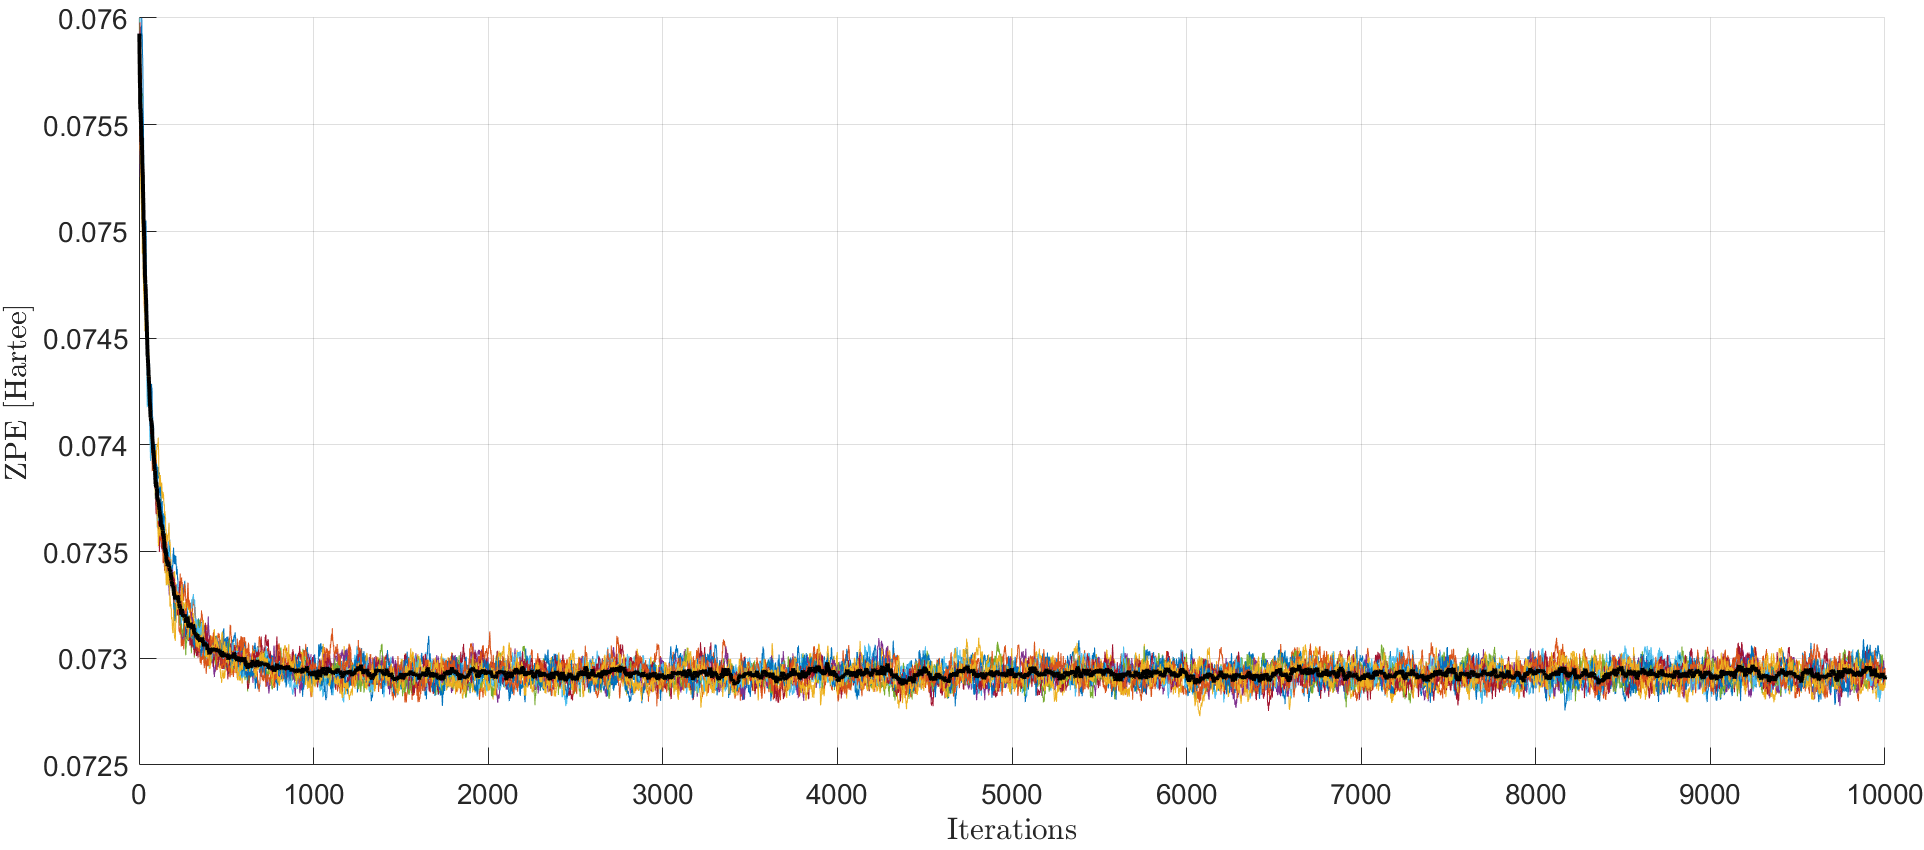
\includegraphics{c2h6_1.png}}\\
Fig. 3. ZPE convergence for $C_2 H_6$. The black line shows the average over the 10 simulations.
\end{center}
ZPE = 0.07293 Hartree with a standard deviation of 0.00002 Hartree. The literature value is 0.073927 Hartree \cite{c2h6}.\\

\end{frame}

\begin{frame}
\frametitle{Results}
\framesubtitle{$C_2 H_6$}
Simulation with 10000 walkers for 10000 time steps
\begin{center}
\scalebox{0.2}{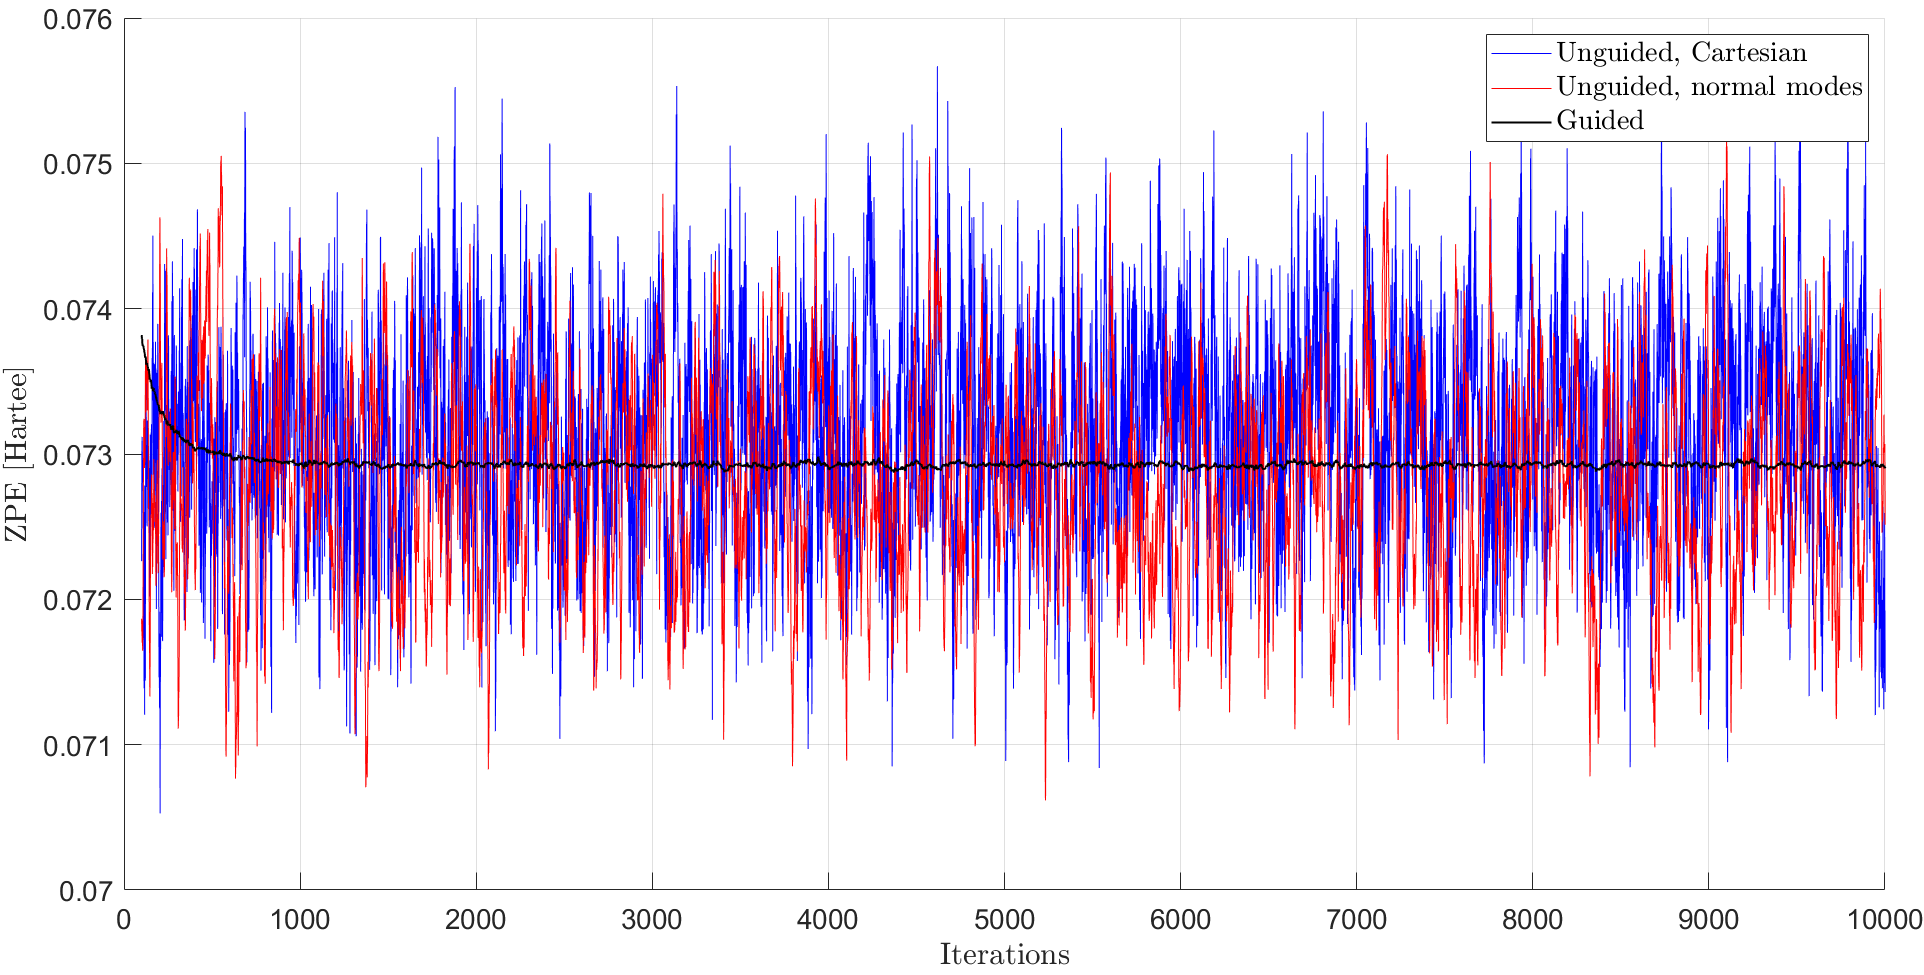
\includegraphics{c2h6_2.png}}\\
Fig. 4. Comparison between guided and unguided DQMC
\end{center}
The fluctuations for unguided DQMC are about 30 to 40 times larger compared to guided DQMC
\end{frame}

\begin{frame}
\frametitle{Results}
\framesubtitle{$C_2 H_6$}
Summary of the results and literature values
\begin{table}[h]
\centering
 \begin{tabular}{||c | c | c||} 
 \hline
 Method & $\overline{ZPE}$ [Hartree] & $\Delta ZPE$ [Hartree] \\ [0.5ex] 
 \hline\hline
 Harmonic approximation & $0.07264$ & \\
 \hline
 Unguided, Cartesian & $0.07322$ &  $0.00076$\\
  \hline
 Unguided, normal modes & $0.07288$ &  $0.00062$\\
 \hline
 Guided & $0.07293$ & $0.00002$ \\
 \hline
 Ref. \cite{c2h6} & $0.07393$ &\\
 \hline
 CCCBDB experimental & $0.07223$ & \\
 \hline
 CCCBDB calculated & $0.07 - 0.08$ & \\
 \hline
\end{tabular}
\end{table}
The guided DQMC needs about a fifth of the simulation time to get the same statistical uncertainty as the unguided DQMC. 
\end{frame}

\subsection{$C_{60}$}

\begin{frame}
\frametitle{Results}
\framesubtitle{$C_{60}$}
\begin{center}
\scalebox{0.30}{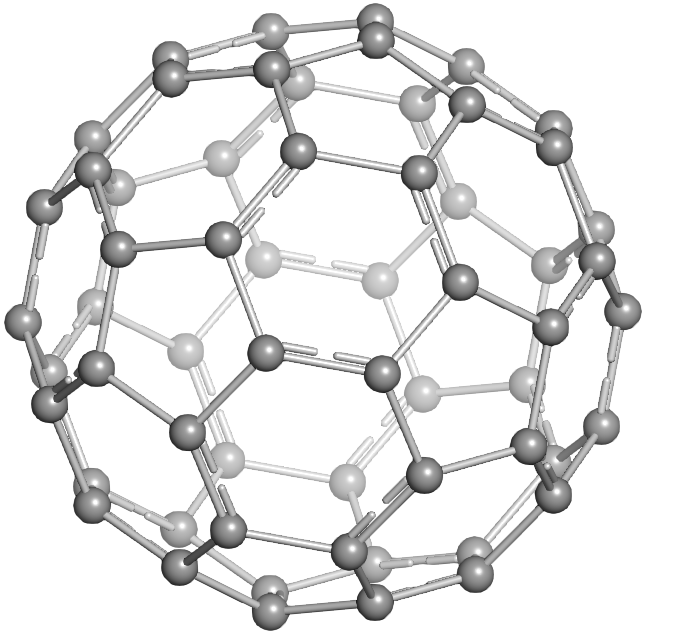
\includegraphics{c60.png}}\\
Fig. 5. Input structure of the $C_{60}$ Buckminsterfullerene
\end{center}
Show the scaling of the algorithm for larger molecules.
\end{frame}

\begin{frame}
\frametitle{Results}
\framesubtitle{$C_{60}$}
10 simulations with 1000 walkers for 10000 time steps
\begin{center}
\scalebox{0.2}{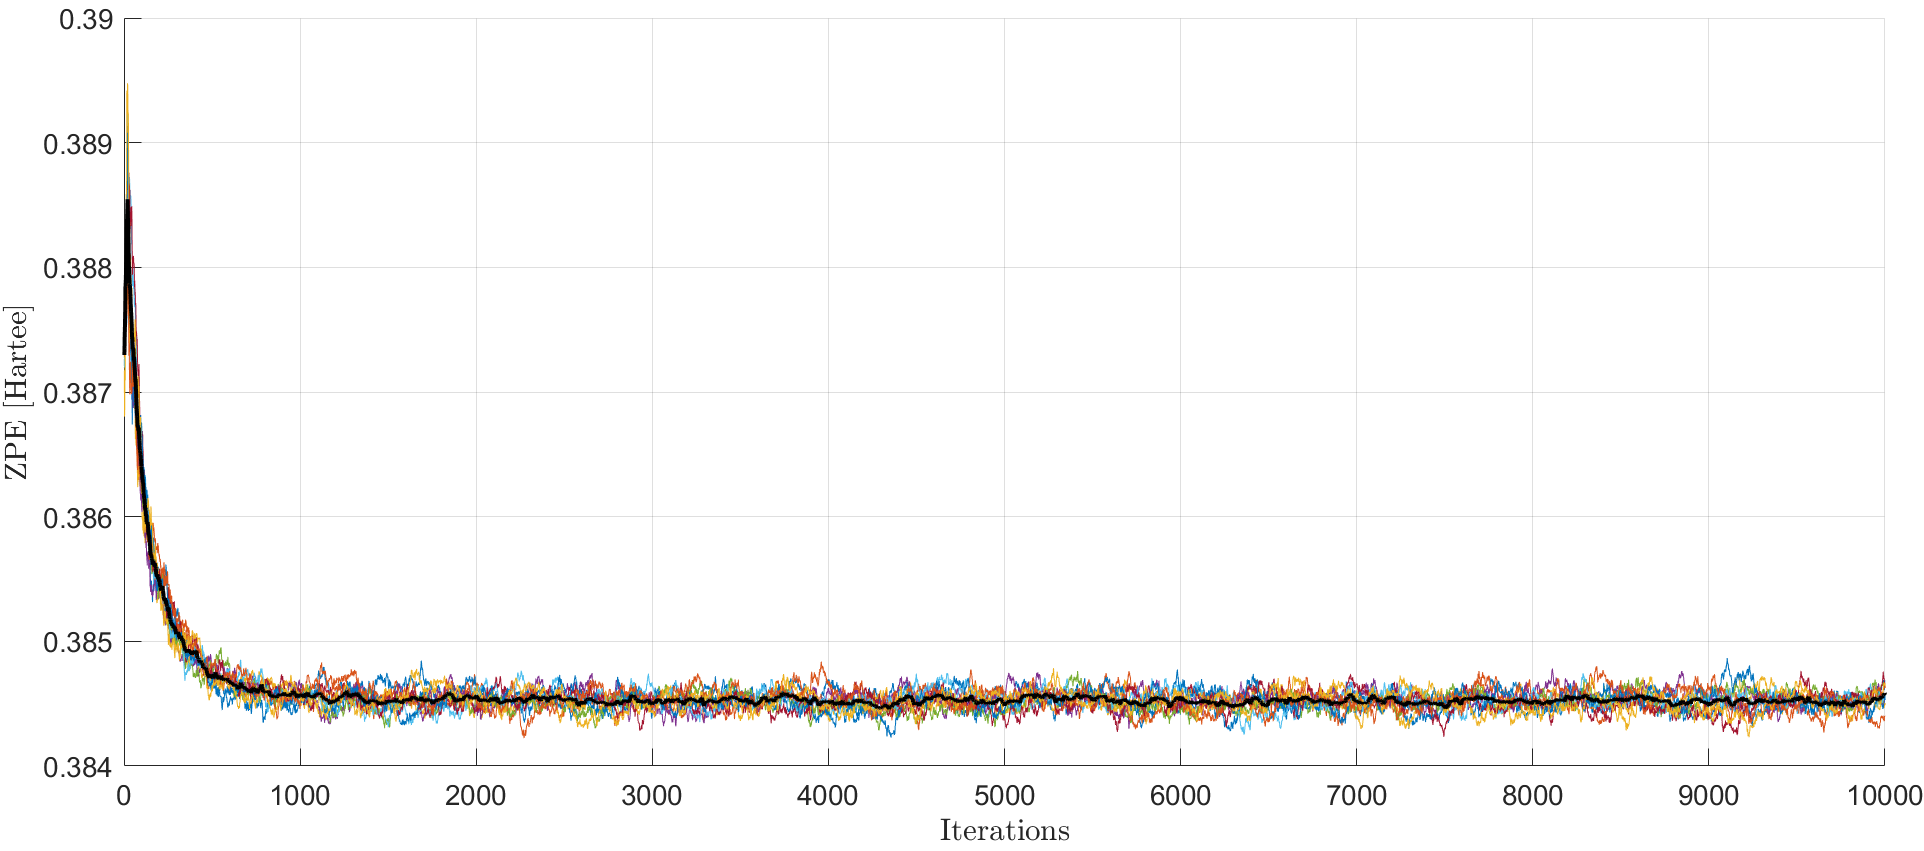
\includegraphics{c60_1.png}}\\
Fig. 3. ZPE convergence for $C_2 H_6$. The black line shows the average over the 10 simulations.
\end{center}
The convergence behavior is similar to $C_2H_6$. We get a ZPE of 0.384524 Hartree with an uncertainty of 0.000014 Hartree. The harmonic approximation gave 0.381769 Hartree.
\end{frame}


\subsection{$H_2@C_{60}$}

\begin{frame}
\frametitle{Results}
\framesubtitle{$H_2@C_{60}$}
\begin{center}
\scalebox{0.3}{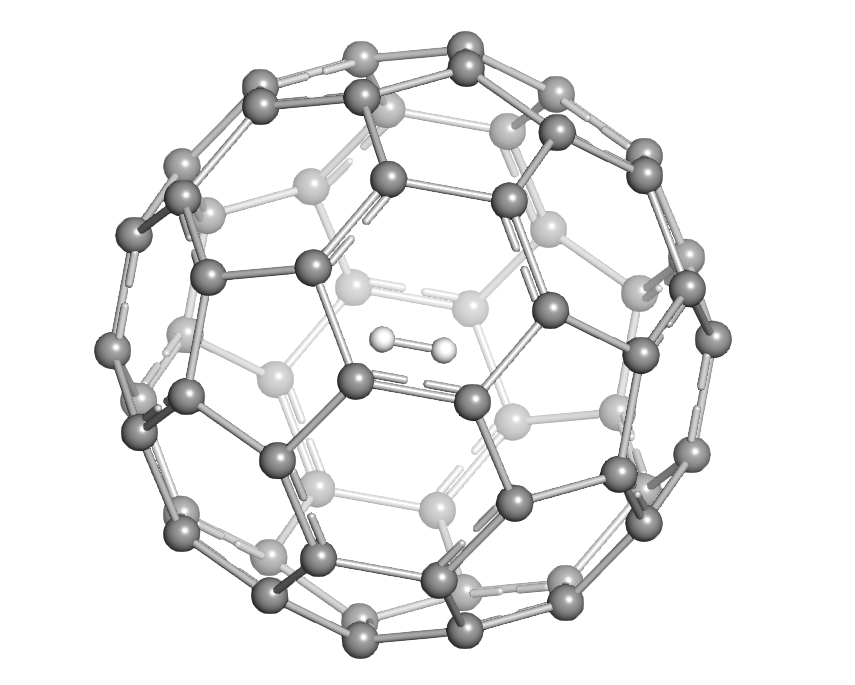
\includegraphics{p3.png}}\\
Fig. 5. Input structure of the $C_{60}$ Buckminsterfullerene
\end{center}
The endohedral hydrogen fullerene shows strong anharmonic effects on the ZPE.\\
\end{frame}

\begin{frame}
\frametitle{Results}
\framesubtitle{$H_2@C_{60}$}
The harmonic approximation fails for the $H_2@C_{60}$.
\begin{center}
\scalebox{0.4}{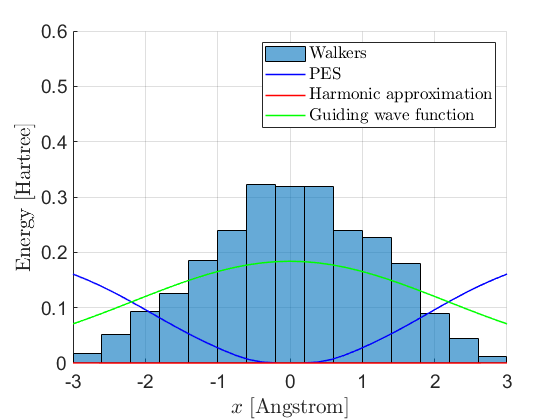
\includegraphics{trialwf_2.png}}\\
Fig. 5. Softest vibrational mode of the  $H_2@C_{60}$
\end{center}
\end{frame}

\begin{frame}
\frametitle{Results}
\framesubtitle{$H_2@C_{60}$}
Simulation with 1000 walkers for 250000 time steps
\begin{center}
\scalebox{0.4}{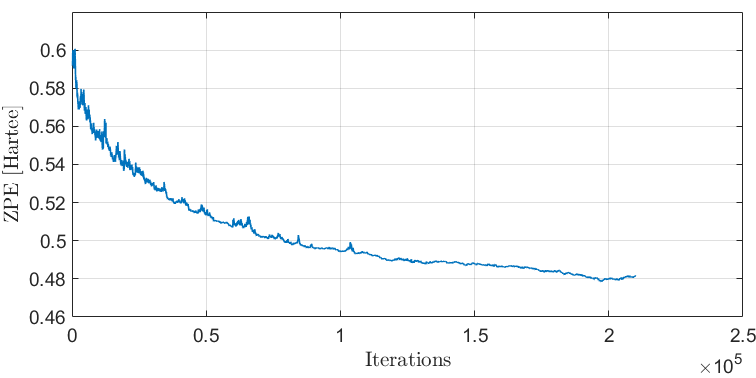
\includegraphics{h2c60_1.png}}\\
Fig. 9. ZPE convergence of $H_2@C_{60}$ (simulation still running)
\end{center}
ZPE $\approx$ 0.48 Hartree which is significantly higher than the harmonic approximation of 0.3984 Hartree.

\end{frame}

\begin{frame}
\frametitle{Results}
\framesubtitle{$H_2@C_{60}$}
\begin{center}
\scalebox{0.25}{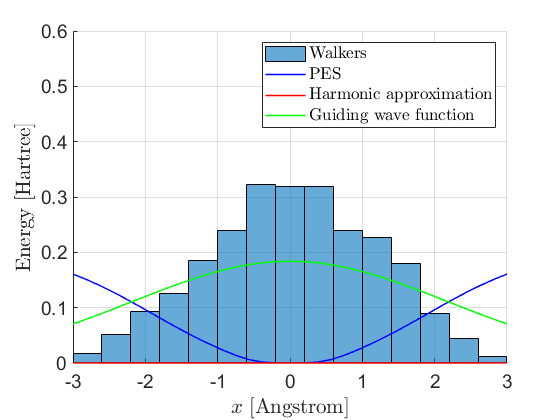
\includegraphics{walkers4.png}}\\
Fig. 10. Final positions of the walkers after the simulation.
\end{center}
\end{frame}

\section{Conclusions}
\begin{frame}
\frametitle{Conclusions}
\begin{itemize}
\item DQMC is a very stable and versatile method to calculate the ZPE
\item The convergence does not depend on the size of the system but on how good the harmonic approximation is. 
\item For $C_2H_6$ and $C_{60}$ the harmonic approximation is good and we converge within 2000 steps.
\item For $H_2@C_{60}$ the harmonic approximation fails and we need 200000 steps to converge. 
\end{itemize}
\end{frame}

\section{Further Research}
\begin{frame}
\frametitle{Further Research}
Marco will continue our work on guided DQMC, adapt the algorithm to periodic structures and compute ZPEs for molecular crystals.
\end{frame}


\begin{frame}
\frametitle{References}
\bibliographystyle{unsrt}
\begin{scriptsize}
\bibliography{references}
\end{scriptsize}
\end{frame}

\end{document}